\documentclass[12pt]{article}
\usepackage[T1]{fontenc}
\usepackage{charter}
\usepackage[scaled=0.92]{helvet}
\usepackage[a4paper,landscape,top=14mm,bottom=14mm,left=16mm,right=16mm,headsep=0mm,headheight=0mm,footskip=8mm]{geometry}
\usepackage{microtype}
\usepackage{enumitem,tabularx,booktabs,array,graphicx,lastpage,fancyhdr,tikz}
\usepackage[table]{xcolor}
\usepackage[hidelinks]{hyperref}
\usepackage{caption}
\usetikzlibrary{positioning,arrows.meta}

\definecolor{accent}{HTML}{1F3F7A}
\definecolor{soft}{HTML}{F3F5F8}
\definecolor{mute}{HTML}{6B7180}
\definecolor{line}{HTML}{D5D9E0}
\setlength{\parindent}{0pt}
\setlength{\parskip}{3pt}
\linespread{1.08}
\pagestyle{fancy}\fancyhf{}
\renewcommand{\headrulewidth}{0pt}
\fancyfoot[L]{\footnotesize\sffamily\color{mute}DongGeon (Lloyd) Kwak \textbullet\ Research Portfolio}
\fancyfoot[R]{\footnotesize\sffamily\color{mute}\thepage\ / \pageref{LastPage}}
\setlist[itemize]{leftmargin=12pt,topsep=1pt,itemsep=2pt,parsep=0pt,label={\small\textbullet}}
\captionsetup{font={small,it},labelformat=empty,skip=4pt}

\newcommand{\kw}[1]{{\setlength{\fboxsep}{4pt}\colorbox{soft}{\sffamily\normalsize\strut #1}}}
\newcommand{\kicker}[1]{{\sffamily\bfseries\footnotesize\color{accent}\MakeUppercase{#1}}\par\vspace{2pt}}
\newcommand{\ptitle}[1]{{\sffamily\bfseries\fontsize{22}{26}\selectfont #1}\par\vspace{12pt}}
\newcommand{\head}[1]{\par\vspace{7pt}{\sffamily\bfseries\scriptsize\color{mute}\MakeUppercase{#1}}\par\vspace{1pt}}
\newcommand{\bignum}[2]{\begin{minipage}[t]{0.47\linewidth}{\sffamily\bfseries\fontsize{19}{22}\selectfont #1}\\[1pt]{\footnotesize\color{mute}#2}\end{minipage}}
\newcommand{\mine}[1]{\par\vspace{8pt}\colorbox{soft}{\parbox{\dimexpr\linewidth-2\fboxsep}{\small{\sffamily\bfseries\scriptsize\color{accent}MY ROLE}\\[1pt]#1}}}

\begin{document}\large

% ======================================================= COVER
\thispagestyle{empty}
\vspace*{22mm}
\begin{minipage}[t]{0.46\linewidth}\vspace{0pt}
  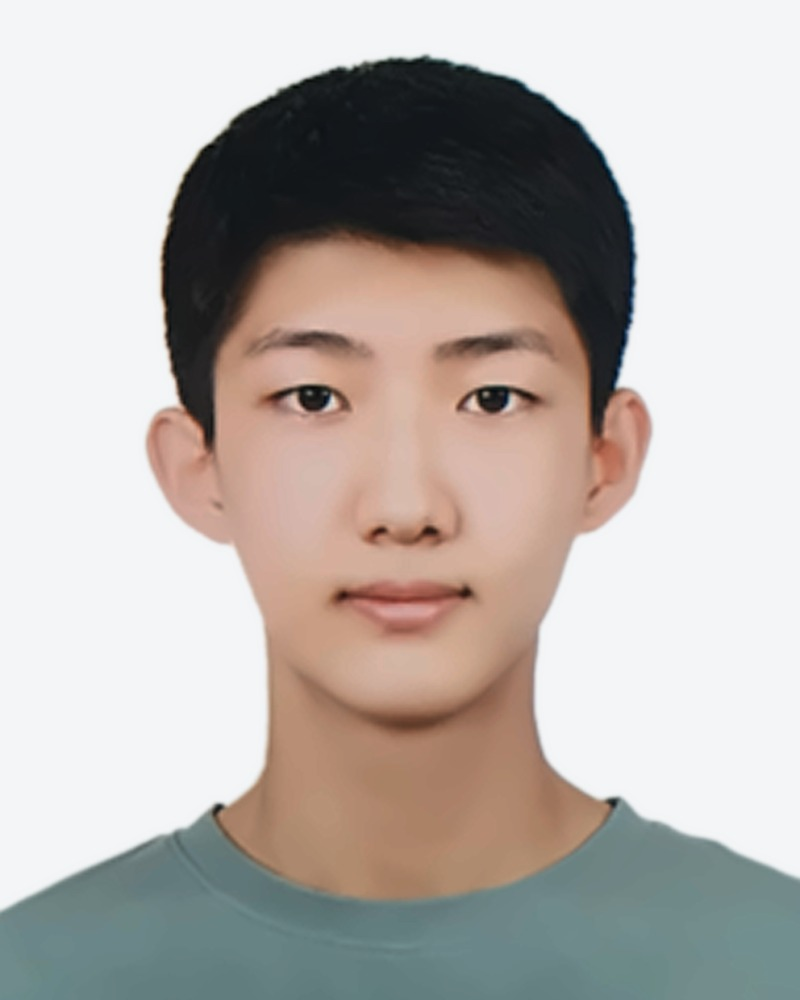
\includegraphics[width=36mm]{profile.jpg}\\[10pt]
  {\sffamily\bfseries\footnotesize\color{accent}RESEARCH PORTFOLIO \textbullet\ 2026}\\[4pt]
  {\sffamily\bfseries\fontsize{30}{34}\selectfont DongGeon (Lloyd) Kwak}\\[8pt]
  {\large B.E.\ Computer Science and Engineering, SeoulTech}\\[2pt]
  {\large Undergraduate Researcher, HCIR Lab (Prof.\ Ji-Hyeong Han)}\\[10pt]
  {\small\color{mute}kwaklloyd@gmail.com \;\textbullet\; lloydkwak.github.io \;\textbullet\; github.com/lloydkwak}
\end{minipage}\hfill
\begin{minipage}[t]{0.47\linewidth}\vspace{2mm}
  {\sffamily\bfseries\scriptsize\color{mute}RESEARCH INTERESTS}\par\vspace{5pt}
  \kw{Generalist robot learning}\\[6pt]
  \kw{Cross-embodiment learning}\\[6pt]
  \kw{Lifelong robot learning: adaptation, failure detection and recovery}\\[6pt]
  \kw{Long-horizon manipulation and task and motion planning}\par
  \vspace{6mm}
  {\sffamily\bfseries\scriptsize\color{mute}CONTENTS}\par\vspace{3pt}
  \renewcommand{\arraystretch}{1.3}
  \begin{tabularx}{\linewidth}{@{}X r@{}}
    \textbf{FAVOR} \; {\color{mute}joint-failure correction} & 2--3\\
    \textbf{MTREA} \; {\color{mute}fine-tuning on a new arm} & 4\\
    \textbf{MakeYourBrick} \; {\color{mute}photo to LEGO model} & 5\\
    \textbf{RL-Arena, image detection} & 6\\
    \textbf{Logisim MLP, work experience} & 7\\
  \end{tabularx}
\end{minipage}

\newpage
% ======================================================= FAVOR 1
\kicker{1 \enspace FAVOR \textbullet\ Jul.\ 2025 -- present \textbullet\ HCIR Lab, SeoulTech}
\ptitle{FAVOR: correcting a diffusion policy after a joint failure}
\begin{minipage}[t]{0.33\linewidth}\vspace{0pt}
  \head{Question}
  When one joint of a robot arm locks or loses range, can a pretrained diffusion policy still finish its task without retraining?
  \head{What I did}
  \begin{itemize}
    \item Injected locked and range-limited faults into a Franka Panda running a diffusion policy (4 LIBERO tasks, 7 joints, 4 severities)
    \item Compared 7 corrections at 3 stages of inference on paired seeds
    \item Found that restoring end-effector position first (priority IK) works best from moderate faults on, and explained why
  \end{itemize}
  \head{Role}
  Sole researcher, advised by Prof.\ Ji-Hyeong Han. First-author manuscript in preparation.
\end{minipage}\hfill
\begin{minipage}[t]{0.63\linewidth}\vspace{0pt}
  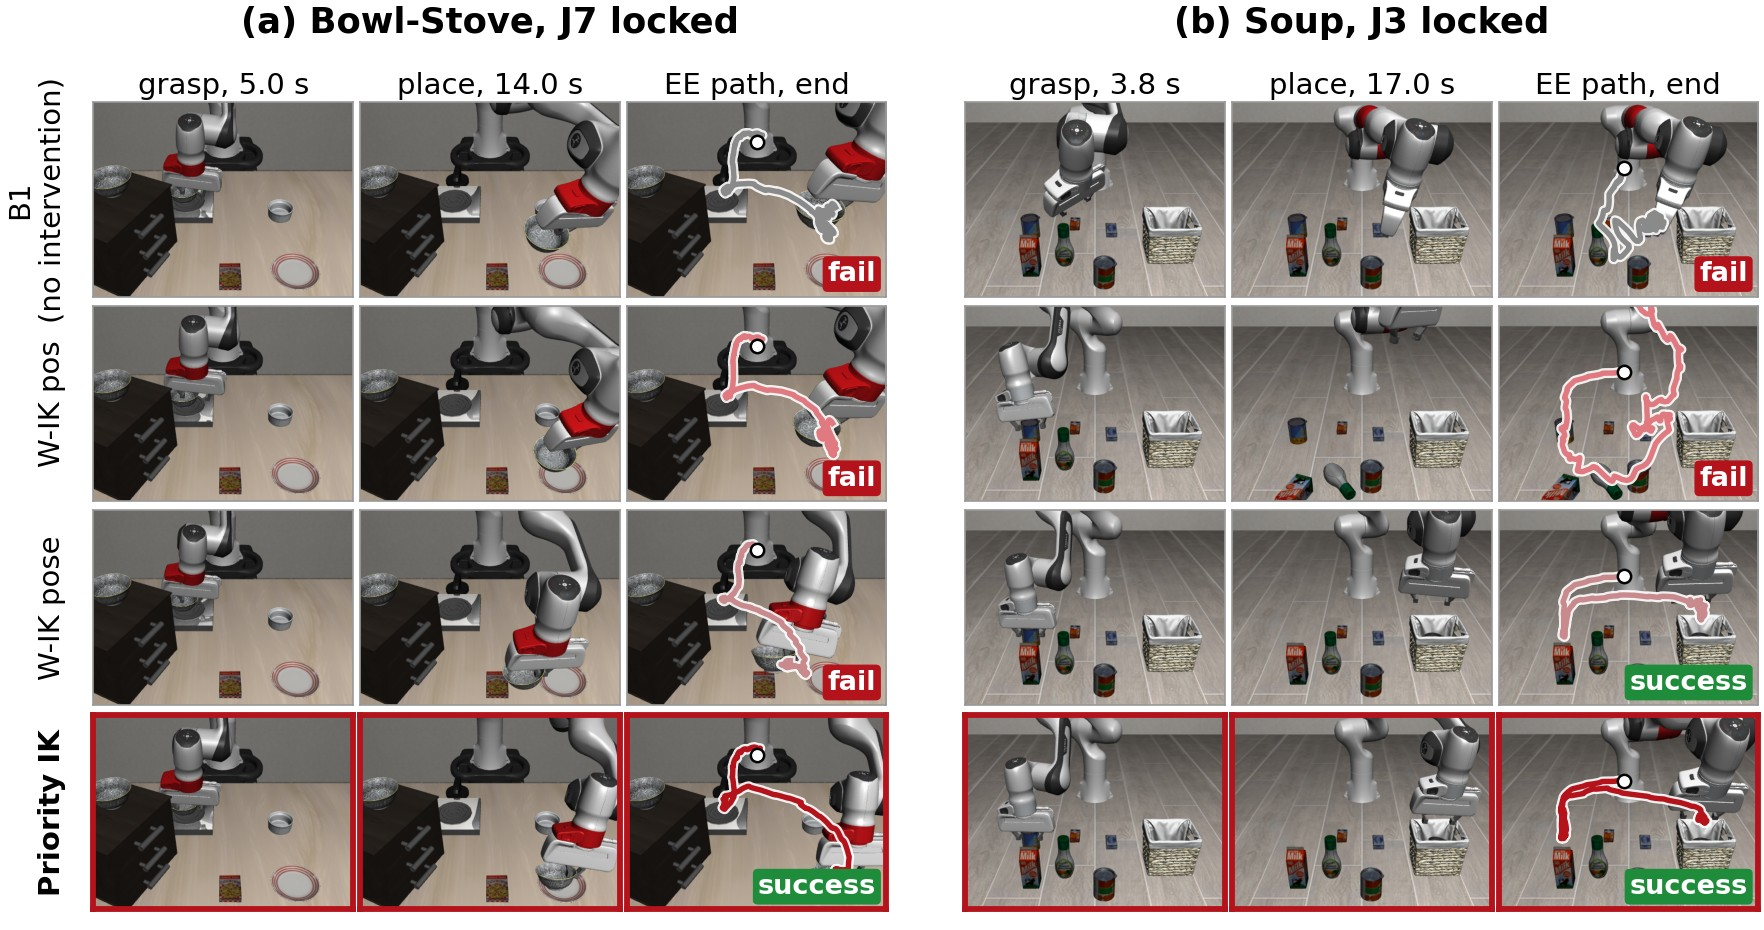
\includegraphics[width=\linewidth]{fig_qual.jpg}
  \captionof{figure}{The same episode under four methods for two faults. Only the bottom row (Priority IK) succeeds in both.}
\end{minipage}

\newpage
% ======================================================= FAVOR 2
\kicker{1 \enspace FAVOR \textbullet\ results}
\ptitle{Correcting position first worked best from moderate faults on}
\begin{minipage}[t]{0.30\linewidth}\vspace{0pt}
  \bignum{0.37 $\to$ 0.60}{mean success,\\112 conditions}\hfill
  \bignum{0.11 $\to$ 0.48}{with a locked\\joint}\\[10pt]
  \bignum{0.94}{AUC: residual error\\predicts recovery}\hfill
  \bignum{0.69}{joint locks\\mid-task}
  \head{Limitations}
  \begin{itemize}
    \item Needs an accurate lock angle (0.01\,rad error: 0.67 $\to$ 0.39)
    \item Locked joints 2 and 4 cannot be compensated
    \item Simulation only so far; real xArm7 tests in progress
  \end{itemize}
\end{minipage}\hfill
\begin{minipage}[t]{0.66\linewidth}\vspace{0pt}
  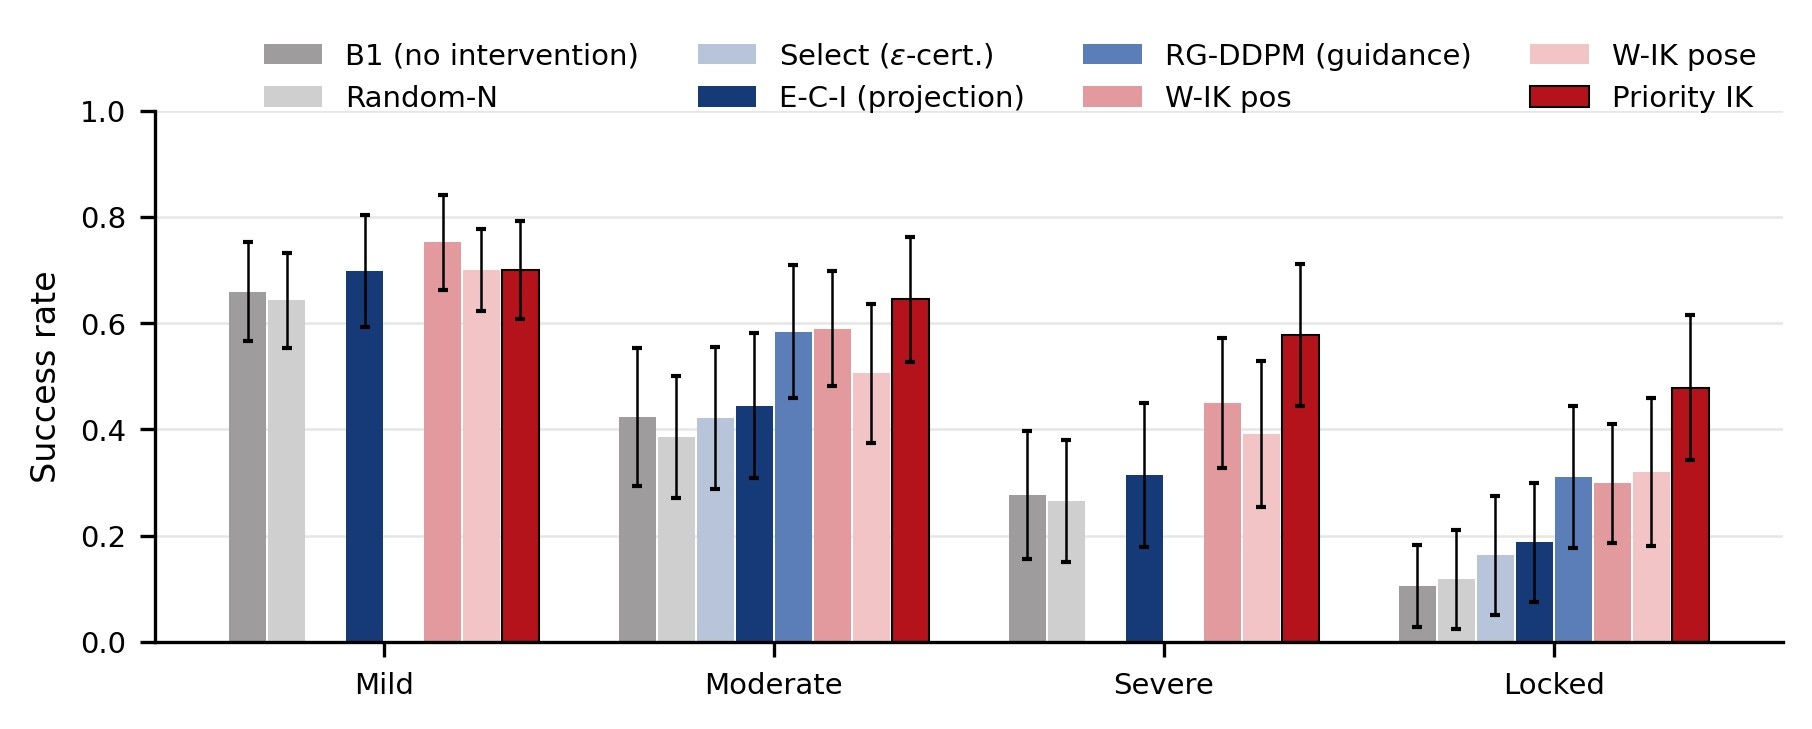
\includegraphics[width=\linewidth]{fig_methods.jpg}
  \captionof{figure}{Success rate by fault level for all methods. Priority IK is dark red.}
  \vspace{4pt}
  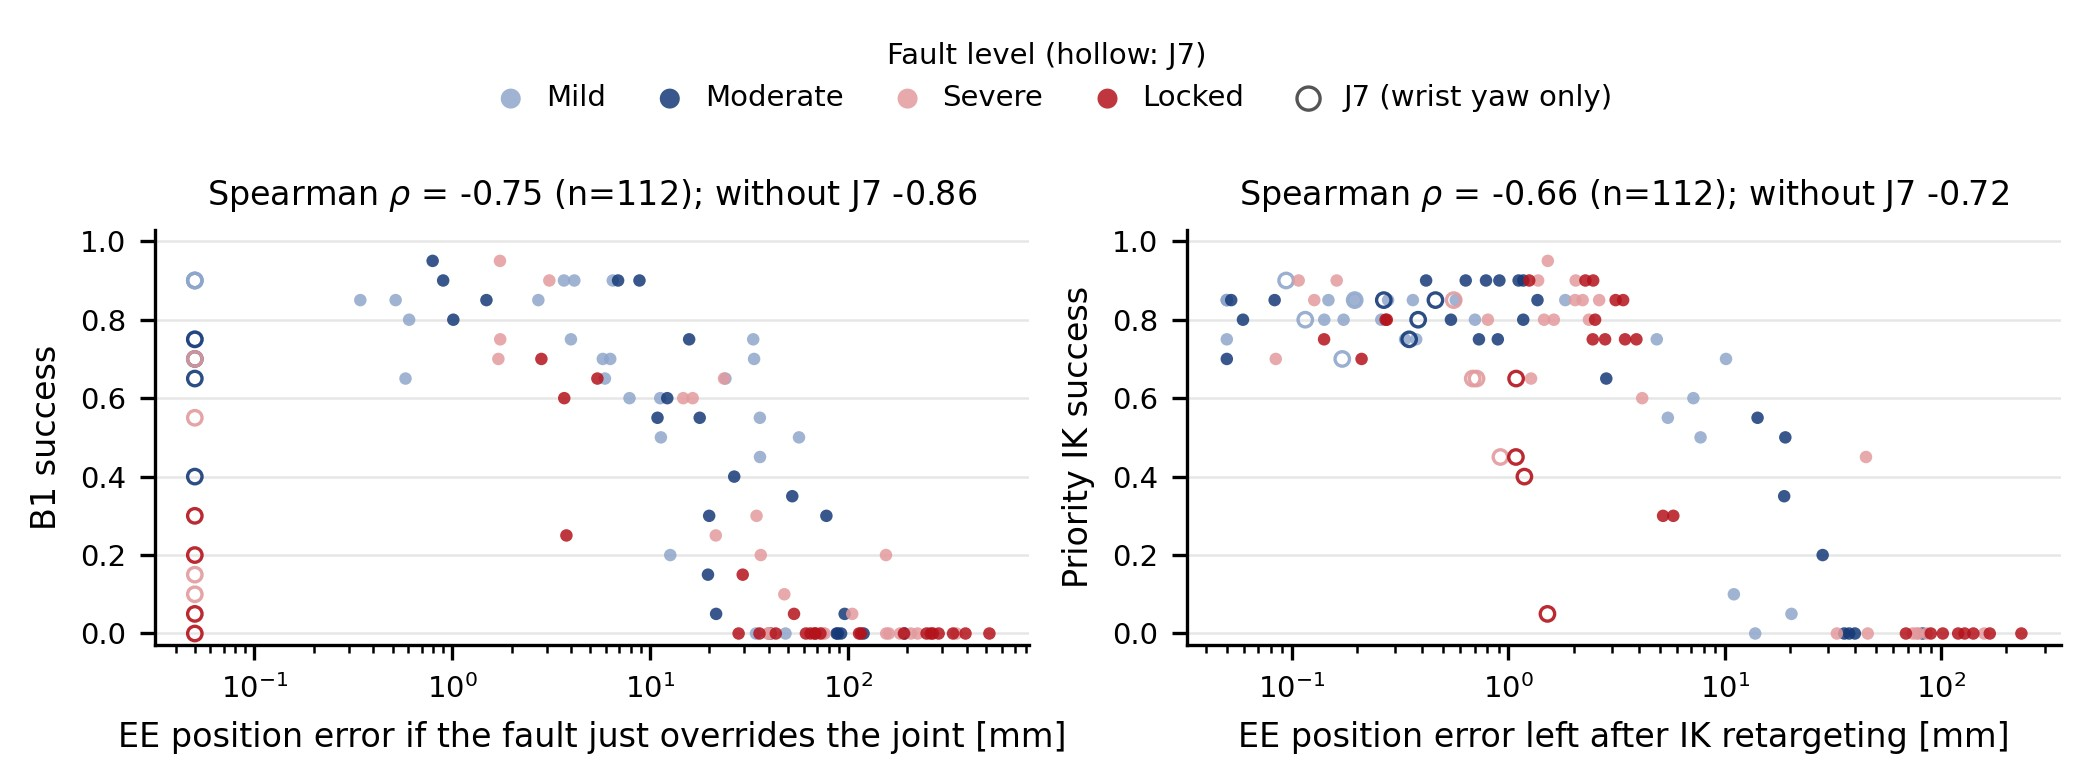
\includegraphics[width=\linewidth]{fig_layer1.jpg}
  \captionof{figure}{Success drops sharply once the end-effector error left after correction exceeds about 10\,mm.}
\end{minipage}

\newpage
% ======================================================= MTREA
\kicker{2 \enspace MTREA \textbullet\ Sep.\ 2026 -- present \textbullet\ Capstone Design \textbullet\ two-person team}
\ptitle{MTREA: does fine-tuning on a new arm reduce other skills?}
\begin{center}
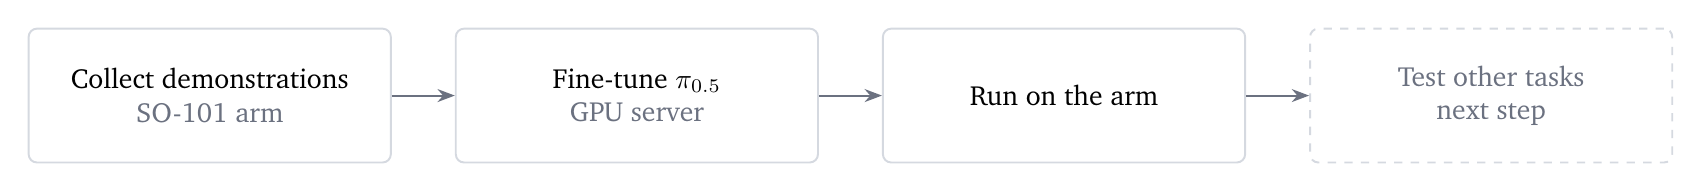
\begin{tikzpicture}[
  box/.style={draw=line,line width=0.7pt,rounded corners=3pt,fill=white,minimum width=46mm,minimum height=17mm,align=center,font=\normalsize},
  nx/.style={box,dashed,text=mute},
  ar/.style={-{Stealth[length=2.2mm]},draw=mute,line width=0.7pt}]
  \node[box] (a) {Collect demonstrations\\{\color{mute}SO-101 arm}};
  \node[box,right=8mm of a] (b) {Fine-tune $\pi_{0.5}$\\{\color{mute}GPU server}};
  \node[box,right=8mm of b] (c) {Run on the arm};
  \node[nx,right=8mm of c] (d) {Test other tasks\\next step};
  \draw[ar] (a)--(b); \draw[ar] (b)--(c); \draw[ar] (c)--(d);
\end{tikzpicture}
\end{center}
\vspace{6pt}
\begin{minipage}[t]{0.47\linewidth}\vspace{0pt}
  \head{Question}
  When $\pi_{0.5}$ is fine-tuned on one task with a new low-cost arm, does it lose performance on tasks it could do before?
  \head{Protocol (with my teammate)}
  Fine-tune on pick-and-place only, then test on other tasks. Naive full fine-tuning is the baseline, since zero-shot stays near zero on a new body; a model fine-tuned on each held-out task is the ceiling.
\end{minipage}\hfill
\begin{minipage}[t]{0.47\linewidth}\vspace{0pt}
  \head{My part}
  Calibration and teleoperation with a safety lock, training on a remote GPU server, and asynchronous serving of the policy on the arm. Chose full fine-tuning at batch 16 from memory measurements on a 40\,GB GPU slice.
  \head{Status}
  The pipeline works end to end. Evaluation on the other tasks is next.
\end{minipage}

\vfill
{\sffamily\bfseries\scriptsize\color{mute}HELD-OUT TASKS, ORDERED BY EXPECTED MOTION OVERLAP WITH THE FINE-TUNING TASK}\par\vspace{6pt}
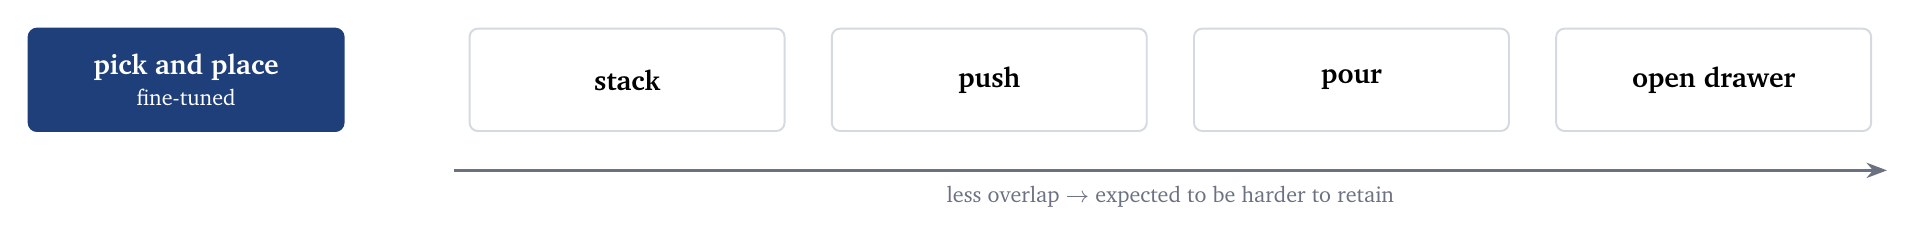
\begin{tikzpicture}[
  t/.style={draw=line,line width=0.7pt,rounded corners=3pt,minimum width=40mm,minimum height=13mm,align=center,font=\normalsize,fill=white},
  f/.style={t,draw=accent,fill=accent,text=white}]
  \node[f] at (0,0) {\textbf{pick and place}\\[-1pt]{\footnotesize fine-tuned}};
  \node[t] at (5.6,0) {\textbf{stack}};
  \node[t] at (10.2,0) {\textbf{push}};
  \node[t] at (14.8,0) {\textbf{pour}};
  \node[t] at (19.4,0) {\textbf{open drawer}};
  \draw[-{Stealth[length=2.6mm]},line width=0.9pt,color=mute] (3.4,-1.15) -- (21.6,-1.15) node[midway,below=2pt,font=\footnotesize,text=mute] {less overlap $\to$ expected to be harder to retain};
\end{tikzpicture}
\vspace*{2mm}

\newpage
% ======================================================= MAKEYOURBRICK
\kicker{3 \enspace MakeYourBrick \textbullet\ May 2026 \textbullet\ SeoulTech startup club}
\ptitle{MakeYourBrick: from a photo to a LEGO model}
\begin{minipage}[t]{0.33\linewidth}\vspace{0pt}
  A web app that turns a single photo into a LEGO model.
  \head{How it works}
  \begin{itemize}
    \item The user selects an object
    \item SAM2 segments it
    \item SAM 3D Objects reconstructs it in 3D
    \item The shape is converted into colored bricks (LDraw format)
  \end{itemize}
  \head{Problem I fixed}
  Shadows in the reconstructed texture turned into black bricks; softening shadows before color quantization removed them.
  \head{Result}
  The model shown uses 10,263 bricks.
\end{minipage}\hfill
\begin{minipage}[t]{0.63\linewidth}\vspace{0pt}\centering
  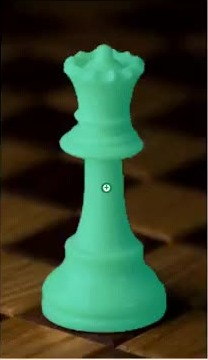
\includegraphics[height=112mm]{myb_demo_crop.jpg}\hspace{4mm}
  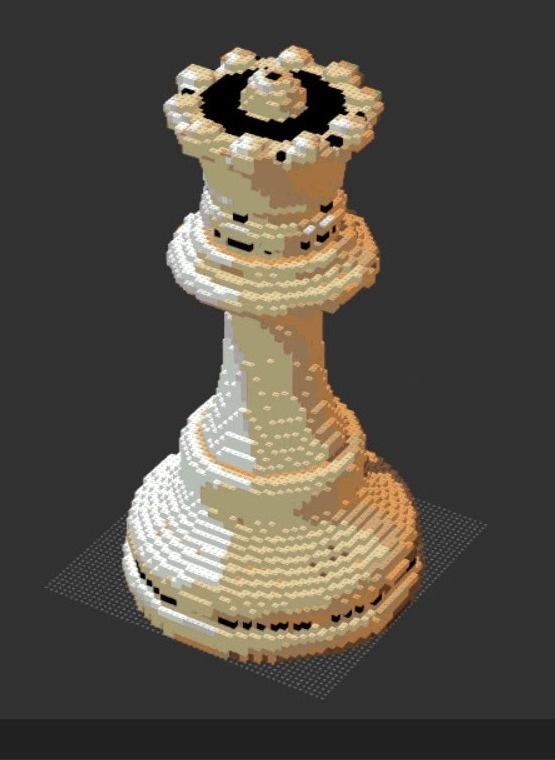
\includegraphics[height=112mm]{myb_ldr_crop.jpg}
  \captionof{figure}{Input photo and the generated model.}
\end{minipage}

\newpage
% ======================================================= RL-ARENA + DETECTION
\begin{minipage}[t]{0.46\linewidth}\vspace{0pt}
  \kicker{4 \enspace RL-Arena \textbullet\ 2025 \textbullet\ Open Source Software course}
  {\sffamily\bfseries\fontsize{18}{22}\selectfont RL-Arena: a platform for ranking RL agents}\par\vspace{10pt}
  Users train reinforcement-learning agents, submit them, and see them ranked against each other.
  \head{Who built what}
  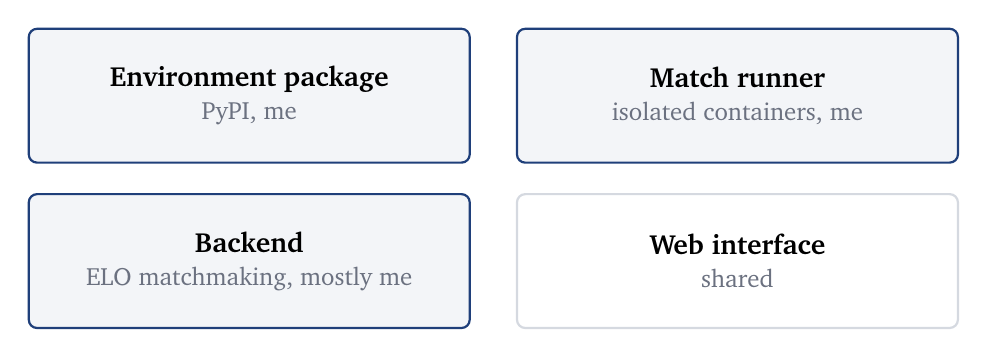
\begin{tikzpicture}[
    m/.style={draw=accent,line width=0.8pt,fill=soft,rounded corners=3pt,minimum width=56mm,minimum height=17mm,align=center,font=\normalsize},
    o/.style={m,draw=line,fill=white}]
    \node[m] at (0,0) {\textbf{Environment package}\\{\small\color{mute}PyPI, me}};
    \node[m] at (6.2,0) {\textbf{Match runner}\\{\small\color{mute}isolated containers, me}};
    \node[m] at (0,-2.1) {\textbf{Backend}\\{\small\color{mute}ELO matchmaking, mostly me}};
    \node[o] at (6.2,-2.1) {\textbf{Web interface}\\{\small\color{mute}shared}};
  \end{tikzpicture}
  \head{Note}
  Two-person team. Selected as an outstanding project in the course.
\end{minipage}\hfill
\begin{minipage}[t]{0.48\linewidth}\vspace{0pt}
  \kicker{5 \enspace AI-generated image detection \textbullet\ 2025 \textbullet\ team of two}
  {\sffamily\bfseries\fontsize{18}{22}\selectfont Detecting images made by diffusion models}\par\vspace{8pt}
  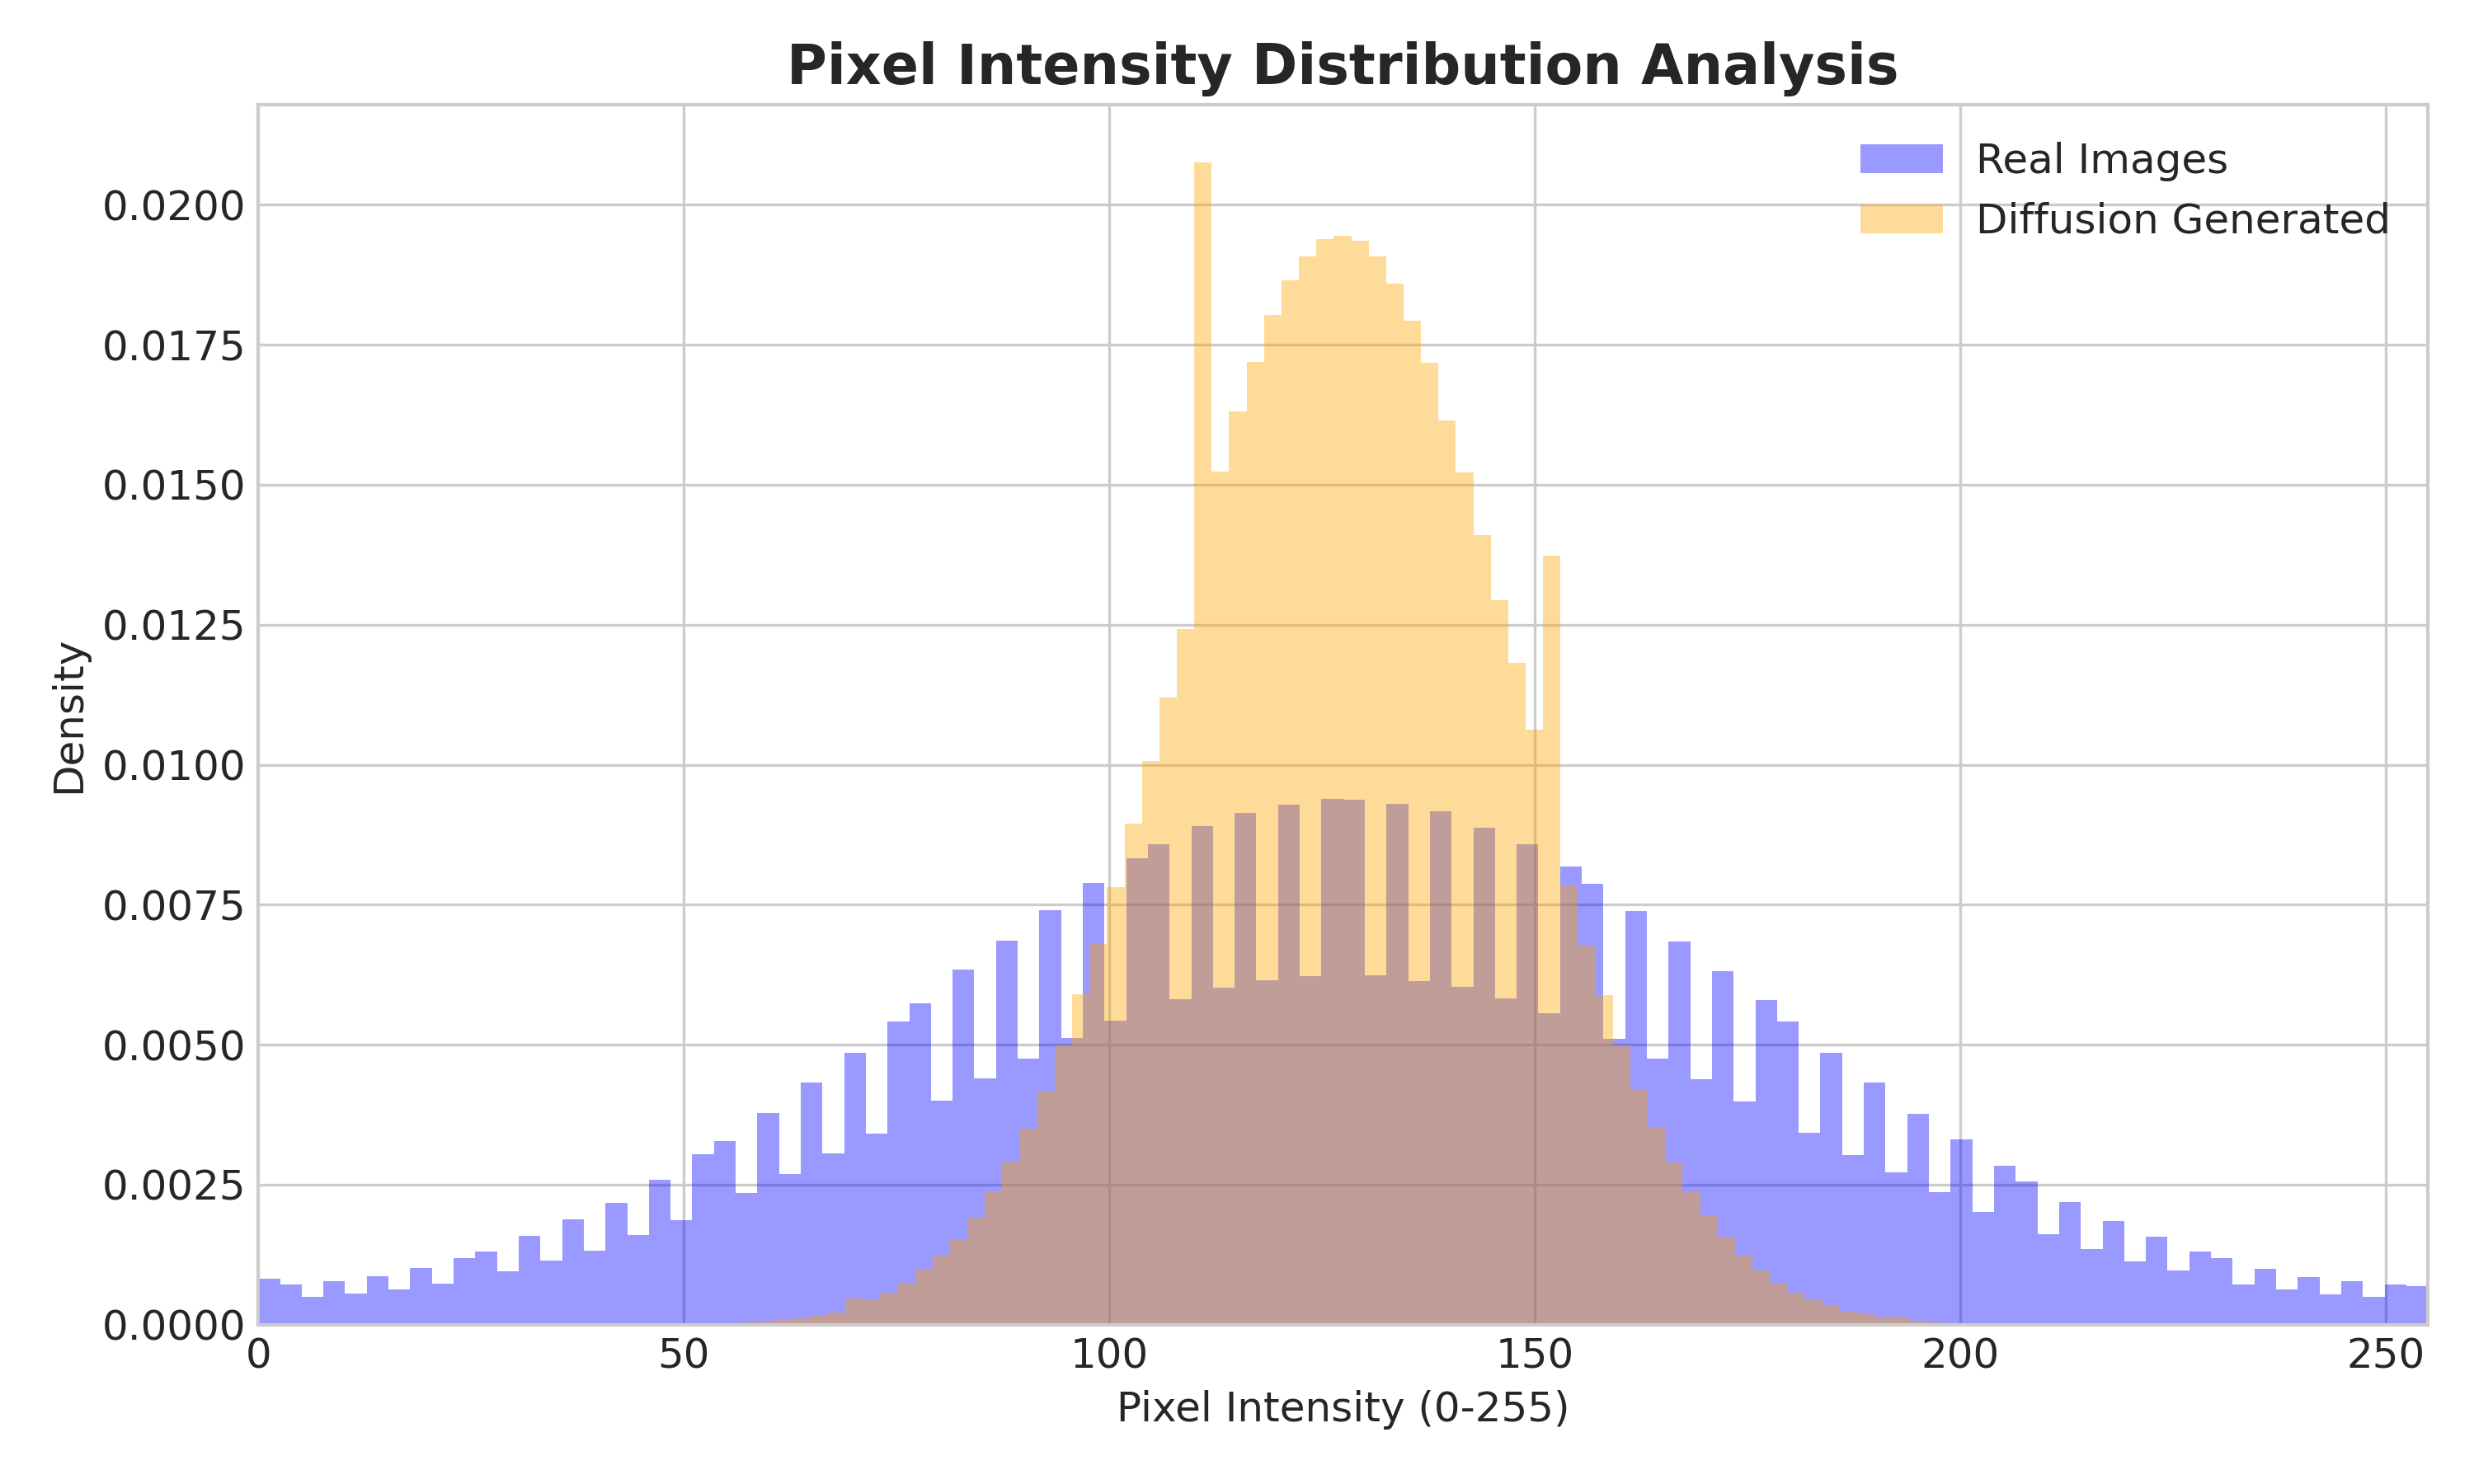
\includegraphics[width=\linewidth]{figure1_pixel_histogram.png}
  \captionof{figure}{Generated images have a narrower spread of pixel intensities than real photos.}
  \vspace{2pt}
  Preprocessing based on this difference raised test accuracy from 72.6\% to 96.3\% (ResNet-50) and from 60.7\% to 88.9\% (EfficientNet-B4) on 115k images.
\end{minipage}

\newpage
% ======================================================= LOGISIM + WORK
\begin{minipage}[t]{0.46\linewidth}\vspace{0pt}
  \kicker{6 \enspace Logisim MLP \textbullet\ 2025 \textbullet\ Digital Logic and Systems course}
  {\sffamily\bfseries\fontsize{18}{22}\selectfont A digit classifier built from logic gates}\par\vspace{8pt}
  \centering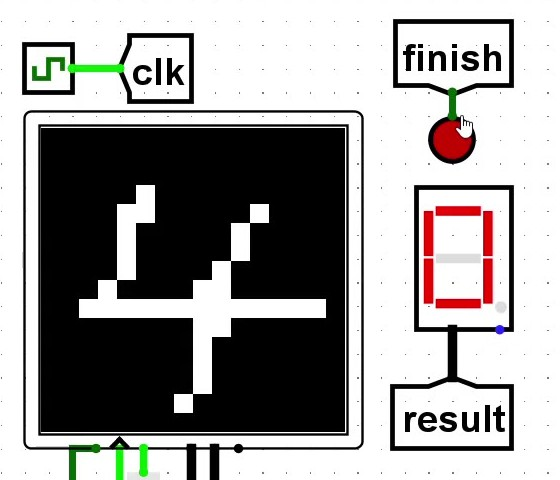
\includegraphics[height=92mm]{logisim.jpg}
  \captionof{figure}{The circuit after classifying a hand-drawn ``4''.}
  \raggedright
  A 256-128-10 MLP with about 34,000 trained weights in ROM, built to understand how a neural network computes at the hardware level. Selected as an outstanding project in the course.
\end{minipage}\hfill
\begin{minipage}[t]{0.48\linewidth}\vspace{0pt}
  \kicker{7 \enspace Work experience \textbullet\ 2022 -- 2023}
  {\sffamily\bfseries\fontsize{18}{22}\selectfont Software developer}\par\vspace{8pt}
  Laver (Jun.\ -- Oct.\ 2022) and CHASER (Nov.\ 2022 -- Jan.\ 2023).
  \begin{itemize}
    \item Object-detection system, from model development to integration
    \item Backend services and APIs
    \item IFC-to-XML converter for building information models
  \end{itemize}
  \head{Patent}
  Co-inventor (third of three) on Korean Patent 10-2647135, \textit{Real-time crack detection system for construction sites}, registered March 2024. Mobile robots record video at construction sites, and cracks are detected and tracked across frames.
\end{minipage}

\end{document}
